\chapter{Angular-Dependent MGXS}
\label{chap:sph}

The results in Chapter~\ref{chap:biases} demonstrated that using the ``true'' flux spectrum from Monte Carlo to perform energy condensation and spatial homogenization will not necessarily result in accurate deterministic multi-group calculations. Large systematic biases in the eigenvalue were observed even for simple heterogeneous benchmark models, and these biases were highly dependent on the energy group structure and spatial discretization used in the multi-group deterministic calculation. In Section~\ref{sec:chap4-diagnosis} it was shown that the bias largely derives from errors in the multi-group reaction rates in the large thermal U-238 capture resonances, and that the errors systematically vary in space within the fuel. These results indicate that one or more of the approximations made in multi-group transport theory are invalidated in heterogeneous geometries and prevents spatial self-shielding at the fuel/moderator interface in \ac{PWR} geometries to be treated appropriately.

Although Chapter~\ref{chap:biases} quantified energy and spatial approximations in multi-group theory, it did not consider the constant-in-angle approximation (see Section~\ref{subsubsec:chap2-const-in-angle}). This chapter reviews some recent work by by Gibson~\cite{gibson2016thesis} to quantify the approximation error resolved with angular dependent \ac{MGXS}, which closely mirrors the trends observed in Chapter~\ref{chap:biases}. The historical \ac{SPH} factor concept is introduced in the context of angular-dependent \ac{MGXS}, and \ac{SPH} factors are applied to simple heterogeneous benchmarks and the results analyzed. Finally, this chapter concludes with a summary of the shortcomings of the \ac{SPH} approach and the need for new methods to account for the angular dependence in \ac{MGXS}.

%Chapter~\ref{chap:mgxs} detailed the approximations made in the multi-group form of the transport equation. 


%%%%%%%%%%%%%%%%%%%%%%%%%%%%%%%%%%%%%%%%%%%%%%%%%%%%%%%%%%%%%%%%%%%%%%%%%%%%%%%
\section{Background}
\label{sec:chap5-background}

The results in Chapter~\ref{chap:biases} demonstrated systematic biases between continuous energy Monte Carlo and deterministic multi-group simulations of simple heterogeneous benchmark models. In Section~\ref{sec:chap4-diagnosis} it was shown that these biases largely derive from errors in the multi-group fluxes/reaction rates in the large thermal U-238 capture resonances. 

-sentence wrapping this paragraph up - talk about spatial self-shielding and segue

These results closely mirror observations by Gibson~\cite{gibson2016thesis} which quantified the errors fundamental to the total 

 illustrated 

\begin{itemize}[noitemsep]
  \item return to angular vs. flux weighting (Section~\ref{subsubsec:chap2-const-in-angle})
  \item Gibson's ``batman'' plot and results
  \item Nelson's 1D slab plot(s)?
\end{itemize}

\cite{gibson2016thesis}


\begin{figure}[H]
\begin{subfigure}{.5\textwidth}
  \centering
  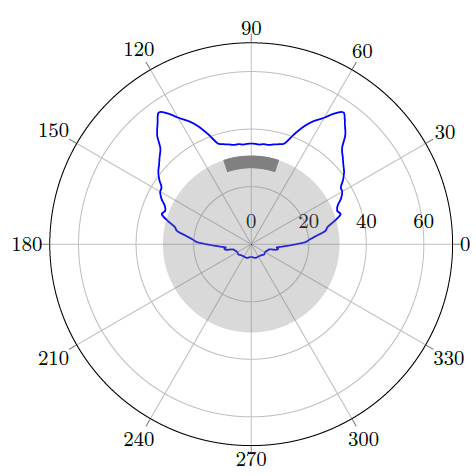
\includegraphics[width=\linewidth]{figures/sph/batman-1}
  \caption{}
\end{subfigure}
\begin{subfigure}{.5\textwidth}
  \centering
  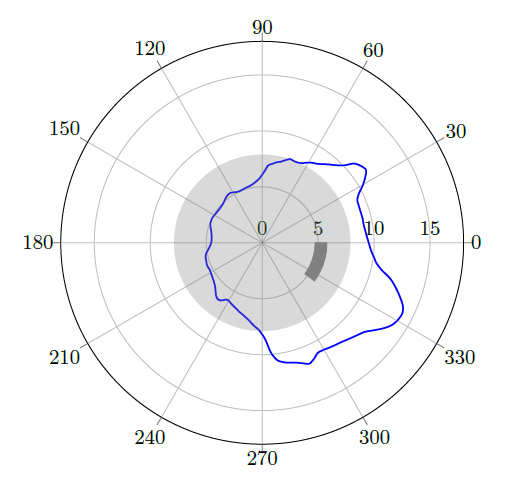
\includegraphics[width=\linewidth]{figures/sph/batman-2}
  \caption{}
\end{subfigure}
\caption[Batman plots]{Cool plots of angular-dependent \ac{MGXS}.}
\label{fig:chap4-rel-err-energy}
\end{figure}

\cite{hebert1993consistent}


%%%%%%%%%%%%%%%%%%%%%%%%%%%%%%%%%%%%%%%%%%%%%%%%%%%%%%%%%%%%%%%%%%%%%%%%%%%%%%%
\section{SuPerHomogenisation Factors}
\label{sec:chap5-sph}

\begin{itemize}
  \item diagnose issue w/ Figures 7.2 and 7.3 from Nate's thesis
  \item introduce basic eqns, reference Hebert
  \item overview algorithm
\end{itemize}


%%%%%%%%%%%%%%%%%%%%%%%%%%%%%%%%%%%%%%%%%%%%%%%%%%%%%%%%%%%%%%%%%%%%%%%%%%%%%%%
\section{SPH Implementation in OpenMOC}
\label{sec:chap5-sph-openmoc}




%%%%%%%%%%%%%%%%%%%%%%
\section{Case Studies}
\label{sec:chap5-sph-results}

%%%%%%%%%%%%%%%%%%%%
\subsection{1D Slab}
\label{subsubsec:chap5-sph-slab}

\begin{itemize}[noitemsep]
  \item plot of fluxes w/ and w/o SPH
  \item plot of Nelson's flux/angular-dependent MGXS???
  \item table of SPH factors in group 27 by group structure
  \item re-generate table of data for slab with bigger moderator
  \item eigenvalues if SPH factors for only group 27 are applied
\end{itemize}

\begin{table}[h!]
  \centering
  \caption{Spatial homogenization error with SPH for a 1D slab.}
  \label{table:chap5-sph-slab-energy} 
  \vspace{14pt}
  \begin{tabular}{c S[table-format=6.1] S[table-format=6.1] S[table-format=6.1] S[table-format=6.1] S[table-format=6.1]}
  \toprule
  & \multicolumn{5}{c}{\boldmath $\Delta\rho$ {\bf [pcm]}} \\
  \midrule  
  \multicolumn{1}{c}{\textbf{\# Groups}} &
  \multicolumn{1}{c}{\bf 1$\times$} &
  \multicolumn{1}{c}{\bf 2$\times$} &
  \multicolumn{1}{c}{\bf 4$\times$} &
  \multicolumn{1}{c}{\bf 8$\times$} &
  \multicolumn{1}{c}{\bf 16$\times$} \\
  \midrule
  & \multicolumn{5}{c}{\bf Without SPH} \\
  \cline{2-6}
1 & 134 & 92 & 121 & 156 & 134 \\
2 & 384 & 228 & 179 & 168 & 165 \\
4 & 236 & 125 & 74 & 57 & 47 \\
8 & 304 & 132 & 39 & -1 & -17 \\
16 & 329 & 136 & 31 & -15 & -32 \\
25 & 247 & 61 & -37 & -81 & -97 \\
40 & 249 & 51 & -56 & -102 & -118 \\
70 & 258 & 51 & -61 & -111 & -123 \\
  \cline{2-6}
  & \multicolumn{5}{c}{\bf With SPH} \\
  \cline{2-6}
1 & 33 & -10 & 18 & 52 & 31 \\
2 & 37 & 13 & 25 & 31 & 13 \\
4 & 16 & 23 & 24 & 28 & 12 \\
8 & 25 & 34 & 24 & 16 & 6 \\
16 & 25 & 35 & 25 & 14 & 3 \\
25 & 26 & 36 & 29 & 20 & 7 \\
40 & 26 & 36 & 27 & 17 & 6 \\
70 & 30 & 38 & 27 & 15 & 7 \\
  \bottomrule
\end{tabular}
\end{table}

\begin{table}[h!]
  \centering
  \caption[SPH factors for a 1D slab]{SPH factors in the energy group encompassing the U-238 capture resonance at 6.67 eV for different energy group structures. The SPH factors were computed for a 1D slab and 2D fuel pin without spatial discretization and with ``iso-in-lab'' scattering.}
  \small
  \label{table:chap5-sph-group-27}
  \vspace{6pt}
  \begin{tabular}{c c S[table-format=2.1] S[table-format=2.1]}
  \toprule
  \multicolumn{1}{c}{\textbf{\# Groups}} &
  \multicolumn{1}{c}{\textbf{Group 27}} &
  \multicolumn{2}{c}{\textbf{SPH Factor $\mu$}} \\
  \midrule
  & & \multicolumn{1}{c}{\bf 1D Slab} &
  \multicolumn{1}{c}{\bf 2D Fuel Pin} \\
  \midrule
1 & & & \\
2 & & & \\
4 & & & \\
8 & & & \\
16 & & & \\
25 & & & \\
40 & & & \\
70 & & & \\
  \bottomrule
\end{tabular}
\end{table}


%%%%%%%%%%%%%%%%%%%%%%%%%%%%%
\subsection{2D Fuel Pin Cell}
\label{subsubsec:chap5-sph-pin}

\begin{itemize}[noitemsep]
  \item table of eigenvalues by energy group w/ and w/o SPH
  \item plot of flux errors with U-238 capture XS w/ and w/o SPH
  \item table of SPH factors in group 27 by energy group structure
\end{itemize}

\begin{table}[h!]
  \centering
  \caption{Spatial homogenization error with SPH for a 2D fuel pin.}
  \label{table:chap5-sph-pin-energy} 
  \vspace{14pt}
  \begin{tabular}{c S[table-format=6.1] S[table-format=6.1] S[table-format=6.1] S[table-format=6.1] S[table-format=6.1]}
  \toprule
  & \multicolumn{5}{c}{\boldmath $\Delta\rho$ {\bf [pcm]}} \\
  \midrule  
  \multicolumn{1}{c}{\textbf{\# Groups}} &
  \multicolumn{1}{c}{\bf 1$\times$} &
  \multicolumn{1}{c}{\bf 2$\times$} &
  \multicolumn{1}{c}{\bf 4$\times$} &
  \multicolumn{1}{c}{\bf 8$\times$} &
  \multicolumn{1}{c}{\bf 16$\times$} \\
  \midrule
  & \multicolumn{5}{c}{\bf Without SPH} \\
  \cline{2-6}
1 & 91 & 92 & 92 & 92 & 92 \\
2 & 153 & 109 & 78 & 67 & 68 \\
4 & 31 & -9 & -38 & -51 & -59 \\
8 & 31 & -29 & -75 & -95 & -106 \\
16 & 41 & -26 & -79 & -103 & -114 \\
25 & -27 & -91 & -142 & -169 & -177 \\
40 & -34 & -103 & -159 & -187 & -196 \\
70 & -35 & -106 & -165 & -195 & -204 \\
  \cline{2-6}
  & \multicolumn{5}{c}{\bf With SPH} \\
  \cline{2-6}
1 & 6 & 6 & 6 & 6 & 6 \\
2 & 32 & 32 & 32 & 32 & 32 \\
4 & 7 & 7 & 7 & 7 & 7 \\
8 & 5 & 5 & 5 & 5 & 5 \\
16 & 6 & 6 & 6 & 6 & 6 \\
25 & 8 & 8 & 8 & 8 & 8 \\
40 & 7 & 7 & 7 & 7 & 7 \\
70 & 8 & 8 & 8 & 8 & 8 \\
  \bottomrule
\end{tabular}
\end{table}


%%%%%%%%%%%%%%%%%%%%%%%%%%%%%%%%%%%%%%%%%%%
%\subsection{2D Heterogeneous Fuel Assembly}
%\label{subsec:chap5-sph-hetero-lat}

%\begin{itemize}[noitemsep]
%  \item table of eigenvalues by energy group w/ and w/o SPH
%  \begin{itemize}[noitemsep]
%    \item cell-avg SPH, region-avg SPH, region-clustered (LNS?) SPH
%  \end{itemize}
%  \item bar chart / rug plot of SPH factors in resonance group(s)
%\end{itemize}

%%%%%%%%%%%%%%%%%%%%%%%
\section{Shortcomings of SPH}
\label{subsec:chap5-sph-shortcomings}
